% move all configuration stuff into one file so we can focus on the content
\documentclass[aspectratio=169,hyperref={pdfpagelabels=false,colorlinks=true,linkcolor=white,urlcolor=lightblue},xcolor={table},t]{beamer}

%%%%%%%%%%%%%%%%%%%%%%%%%%%%%%%%%%%%%%%%%%%%%%%%%%%%%%%%%%%%%%%%%%%%%%%%%%%%%%%%%%
%%%%%%%%%%%%%%%%%%%%%%%%%%%%%%%%%%%%%%%%%%%%%%%%%%%%%%%%%%%%%%%%%%%%%%%%%%%%%%%%%%
% packages
\usepackage{pict2e}
\usepackage{epic}
\usepackage{amsmath,amsfonts,amssymb}
\usepackage{units}
\usepackage{fancybox}
\usepackage[absolute,overlay]{textpos} 
%\usepackage[table]{xcolor}
\usepackage{animate}
\usepackage{gensymb}
%\usepackage{graphicx}
%\usepackage{longtable}
\usepackage{multirow}
\usepackage{silence}
\usepackage{tikz}
\usepackage[backend=bibtex,style=ieee]{biblatex}
\AtEveryCitekey{\iffootnote{\tiny}{}}
%\addbibresource{include/references}



% fontsize
\let\Tiny=\tiny

%%%%%%%%%%%%%%%%%%%%%%%%%%%%%%%%%%%%%%%%%%%%%%%%%%%%%%%%%%%%%%%%%%%%%%%%%%%%%%%%%%
%%%%%%%%%%%%%%%%%%%%%%%%%%%%%%%%%%%%%%%%%%%%%%%%%%%%%%%%%%%%%%%%%%%%%%%%%%%%%%%%%%
% warnings
\pdfsuppresswarningpagegroup=1
\WarningFilter{biblatex}{Patching footnotes failed}
\WarningFilter{latexfont}{Font shape}
\WarningFilter{latexfont}{Some font shapes}
\WarningFilter{gensymb}{Not defining}


%%%%%%%%%%%%%%%%%%%%%%%%%%%%%%%%%%%%%%%%%%%%%%%%%%%%%%%%%%%%%%%%%%%%%%%%%%%%%%%%%%
%%%%%%%%%%%%%%%%%%%%%%%%%%%%%%%%%%%%%%%%%%%%%%%%%%%%%%%%%%%%%%%%%%%%%%%%%%%%%%%%%%
% theme & layout
\usetheme{Frankfurt}
\useinnertheme{rectangles}


%%%%%%%%%%%%%%%%%%%%%%%%%%%%%%%%%%%%%%%%%%%%%%%%%%%%%%%%%%%%%%%%%%%%%%%%%%%%%%%%%%
\setbeamertemplate{frametitle}[default][colsep=-4bp,rounded=false,shadow=false]
\setbeamertemplate{frametitle}
{%
    \nointerlineskip%
    %\vskip-0.5ex
    \begin{beamercolorbox}[wd=\paperwidth,ht=3.5ex,dp=0.6ex]{frametitle}
        \hspace*{1.3ex}\insertframetitle%
        
        \hspace*{1.3ex}\small\insertframesubtitle%
    \end{beamercolorbox}%
    \begin{textblock*}{100mm}(13.75cm,1cm)
        
\includegraphics[height=.4cm,keepaspectratio]{../shared/Logo_GTCMT_white}
    \end{textblock*}
}


%%%%%%%%%%%%%%%%%%%%%%%%%%%%%%%%%%%%%%%%%%%%%%%%%%%%%%%%%%%%%%%%%%%%%%%%%%%%%%%%%%
\setbeamertemplate{title page}[default][colsep=-4bp,rounded=false,shadow=false]
\setbeamertemplate{title page}
{
    %\begin{textblock*}{100mm}(15cm,.51cm)
            %\href{https://github.com/alexanderlerch/ACA-Slides/blob/2nd_edition/\jobname.pdf}{\includegraphics[height=.5cm,keepaspectratio]{graph/Logo_github}}\hspace*{2ex}
    %\end{textblock*}
    %\begin{textblock*}{100mm}(15cm,1.3cm)
            %\href{\IEEELink}{\includegraphics[height=.5cm,keepaspectratio]{graph/icon/book}}\hspace*{2ex}
    %\end{textblock*}
    \vskip-10ex
    \begin{beamercolorbox}[wd=\paperwidth,ht=.7\paperheight,dp=0.6ex]{frametitle} %35ex
        %\begin{flushright}
            %\href{http://www.gtcmt.gatech.edu}{
\includegraphics[height=.8cm,keepaspectratio]{graph/Logo_GTCMT_black}}\hspace*{2ex}
        %\end{flushright}
        
        \hspace*{1.8ex}\LARGE\inserttitle%
        
        \vspace*{.5ex}
        
        \hspace*{1.3ex}\small\insertsubtitle%
        
        \vspace*{.5ex}
    \end{beamercolorbox}%
    \nointerlineskip%
    \begin{beamercolorbox}[wd=\paperwidth,ht=.4\paperheight,dp=0.6ex]{page number in head/foot}
        %\vspace*{-.5ex}
        \hspace*{1.7ex}\small\insertauthor%
        
        %\hspace*{1.7ex}\small }%
        
        \vspace*{12ex}
        \vfill
        \begin{flushright}
            \href{http://www.gtcmt.gatech.edu}{
\includegraphics[height=.5cm,keepaspectratio]{../shared/Logo_GTCMT_black}}\hspace*{2ex}
        \end{flushright}
    \end{beamercolorbox}%
}


%%%%%%%%%%%%%%%%%%%%%%%%%%%%%%%%%%%%%%%%%%%%%%%%%%%%%%%%%%%%%%%%%%%%%%%%%%%%%%%%%%
%\makeatother
\setbeamertemplate{footline}
{
  \leavevmode%
  \hbox{%
  \begin{beamercolorbox}[wd=.5\paperwidth,ht=2.25ex,dp=1ex,left,leftskip=1ex]{page number in head/foot}%
    \insertsubtitle
  \end{beamercolorbox}%
  \begin{beamercolorbox}[wd=.5\paperwidth,ht=2.25ex,dp=1ex,right,rightskip=1ex]{page number in head/foot}%
    \hfill
    \insertframenumber{} / \inserttotalframenumber
  \end{beamercolorbox}}%
  \vskip0pt%
}
%\makeatletter


%%%%%%%%%%%%%%%%%%%%%%%%%%%%%%%%%%%%%%%%%%%%%%%%%%%%%%%%%%%%%%%%%%%%%%%%%%%%%%%%%%
\beamertemplatenavigationsymbolsempty
\setbeamertemplate{navigation symbols}{}
\setbeamertemplate{blocks}[default]%[rounded=false,shadow=false]
\setbeamertemplate{itemize item}[square]
\setbeamertemplate{itemize subitem}[circle]
\setbeamertemplate{itemize subsubitem}[triangle]
\setbeamertemplate{enumerate item}[square]
\setbeamertemplate{enumerate subitem}[circle]
\setbeamertemplate{enumerate subsubitem}[circle]


%%%%%%%%%%%%%%%%%%%%%%%%%%%%%%%%%%%%%%%%%%%%%%%%%%%%%%%%%%%%%%%%%%%%%%%%%%%%%%%%%%
% colors
\setbeamercolor{structure}{fg=darkgray}
\setbeamercovered{transparent} %invisible
\setbeamercolor{bibliography entry author}{fg=black}
\setbeamercolor*{bibliography entry title}{fg=black}
\setbeamercolor*{bibliography entry note}{fg=black}
\setbeamercolor{frametitle}{fg=black}
\setbeamercolor{title}{fg=white}
\setbeamercolor{subtitle}{fg=white}
\setbeamercolor{frametitle}{fg=white}
\setbeamercolor{framesubtitle}{fg=white}
\setbeamercolor{mini frame}{fg=white, bg=black}
\setbeamercolor{section in head/foot}{fg=white, bg=darkgray}
\setbeamercolor{page number in head/foot}{fg=black, bg=gtgold}
\setbeamercolor{item projected}{fg=white, bg=black}

%---------------------------------------------------------------------------------

%%%%%%%%%%%%%%%%%%%%%%%%%%%%%%%%%%%%%%%%%%%%%%%%%%%%%%%%%%%%%%%%%%%%%%%%%%%%%%%%%%
%%%%%%%%%%%%%%%%%%%%%%%%%%%%%%%%%%%%%%%%%%%%%%%%%%%%%%%%%%%%%%%%%%%%%%%%%%%%%%%%%%
% title information
\title[]{MUSI6202: Digital Signal Processing for Music}   
\author[alexander lerch]{alexander lerch} 
%\institute{~}
%\date[Alexander Lerch]{}
%\titlegraphic{\vspace{-16mm}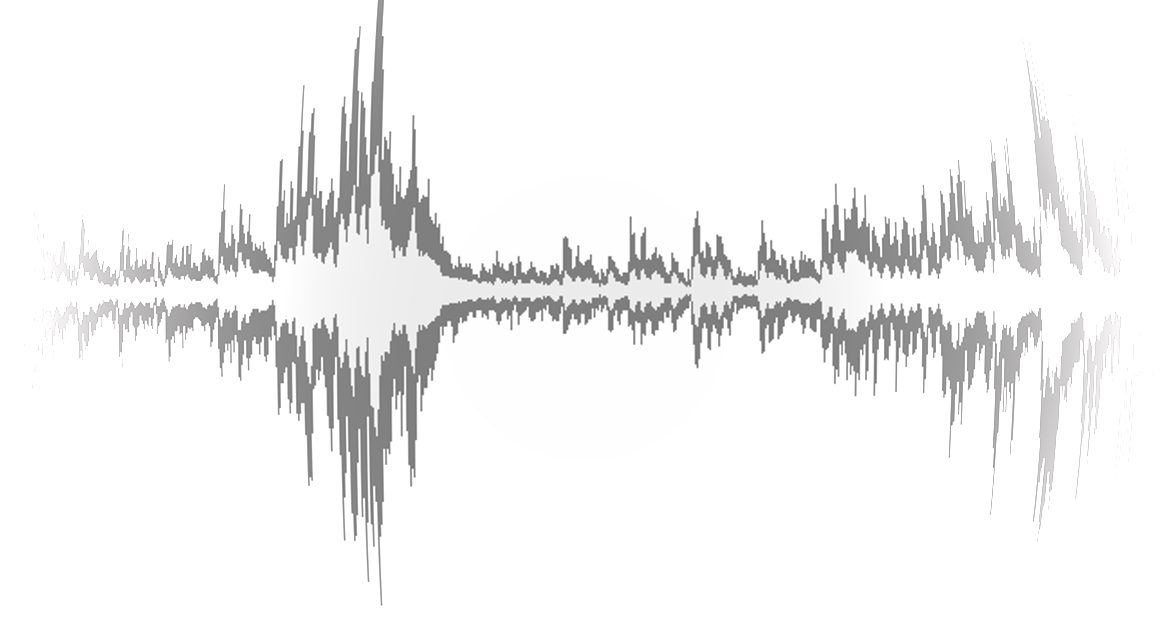
\includegraphics[width=\textwidth,height=3cm]{title}}

%%%%%%%%%%%%%%%%%%%%%%%%%%%%%%%%%%%%%%%%%%%%%%%%%%%%%%%%%%%%%%%%%%%%%%%%%%%%%%%%%%
%%%%%%%%%%%%%%%%%%%%%%%%%%%%%%%%%%%%%%%%%%%%%%%%%%%%%%%%%%%%%%%%%%%%%%%%%%%%%%%%%%
% colors
\definecolor{gtgold}{rgb}{.914, .664, 0} %0e7eed {rgb}{0.88,0.66,1,0.06} [234, 170, 0]/256 %96caff
\definecolor{darkgray}{rgb}{.15, .15, .15}
\definecolor{lightblue}{HTML}{0e7eed}
\definecolor{highlight}{rgb}{0, 0, 1} %_less!40

%%%%%%%%%%%%%%%%%%%%%%%%%%%%%%%%%%%%%%%%%%%%%%%%%%%%%%%%%%%%%%%%%%%%%%%%%%%%%%%%%%
%%%%%%%%%%%%%%%%%%%%%%%%%%%%%%%%%%%%%%%%%%%%%%%%%%%%%%%%%%%%%%%%%%%%%%%%%%%%%%%%%%
% relative paths
\graphicspath{{../graph/}}


%%%%%%%%%%%%%%%%%%%%%%%%%%%%%%%%%%%%%%%%%%%%%%%%%%%%%%%%%%%%%%%%%%%%%%%%%%%%%%%%%%
%%%%%%%%%%%%%%%%%%%%%%%%%%%%%%%%%%%%%%%%%%%%%%%%%%%%%%%%%%%%%%%%%%%%%%%%%%%%%%%%%%
% units
\setlength{\unitlength}{1mm}

%%%%%%%%%%%%%%%%%%%%%%%%%%%%%%%%%%%%%%%%%%%%%%%%%%%%%%%%%%%%%%%%%%%%%%%%%%%%%%%%%%
%%%%%%%%%%%%%%%%%%%%%%%%%%%%%%%%%%%%%%%%%%%%%%%%%%%%%%%%%%%%%%%%%%%%%%%%%%%%%%%%%%
% math
\DeclareMathOperator*{\argmax}{argmax}
\DeclareMathOperator*{\argmin}{argmin}
\DeclareMathOperator*{\atan}{atan}
\DeclareMathOperator*{\arcsinh}{arcsinh}
\DeclareMathOperator*{\sign}{sign}
\DeclareMathOperator*{\tcdf}{tcdf}
\DeclareMathOperator*{\si}{sinc}
\DeclareMathOperator*{\princarg}{princarg}
\DeclareMathOperator*{\arccosh}{arccosh}
\DeclareMathOperator*{\hwr}{HWR}
\DeclareMathOperator*{\flip}{flip}
\DeclareMathOperator*{\sinc}{sinc}
\DeclareMathOperator*{\floor}{floor}
\newcommand{\e}{{e}}
\newcommand{\jom}{\mathrm{j}\omega}
\newcommand{\jOm}{\mathrm{j}\Omega}
\newcommand   {\mat}[1]    		{\boldsymbol{\uppercase{#1}}}		%bold
\renewcommand {\vec}[1]    		{\boldsymbol{\lowercase{#1}}}		%bold

%%%%%%%%%%%%%%%%%%%%%%%%%%%%%%%%%%%%%%%%%%%%%%%%%%%%%%%%%%%%%%%%%%%%%%%%%%%%%%%%%%
%%%%%%%%%%%%%%%%%%%%%%%%%%%%%%%%%%%%%%%%%%%%%%%%%%%%%%%%%%%%%%%%%%%%%%%%%%%%%%%%%%
% media9
\newcommand{\includeaudio}[1]{
\href{run:audio/#1.mp3}{
\includegraphics[width=5mm, height=5mm]{graph/SpeakerIcon}}}

\newcommand{\includeanimation}[4]{{\begin{center}
                        \animategraphics[autoplay,loop,scale=.7]{#4}{animation/#1-}{#2}{#3}        
                        \end{center}
                        \addreference{matlab source: \href{https://github.com/alexanderlerch/ACA-Plots/blob/master/matlab/animate#1.m}{matlab/animate#1.m}}}
                        \inserticon{video}}
                        
%%%%%%%%%%%%%%%%%%%%%%%%%%%%%%%%%%%%%%%%%%%%%%%%%%%%%%%%%%%%%%%%%%%%%%%%%%%%%%%%%%
%%%%%%%%%%%%%%%%%%%%%%%%%%%%%%%%%%%%%%%%%%%%%%%%%%%%%%%%%%%%%%%%%%%%%%%%%%%%%%%%%%
% other commands
\newcommand{\question}[1]{%\vspace{-4mm}
                          \setbeamercovered{invisible}
                          \begin{columns}[T]
                            \column{.9\textwidth}
                                \textbf{#1}
                            \column{.1\textwidth}
                                \vspace{-8mm}
                                \begin{flushright}
                                     
\includegraphics[width=.9\columnwidth]{graph/question_mark}
                                \end{flushright}
                                \vspace{6mm}
                          \end{columns}\pause\vspace{-12mm}}

\newcommand{\toremember}[1]{
                        \inserticon{lightbulb}
                        }

\newcommand{\matlabexercise}[1]{%\vspace{-4mm}
                          \setbeamercovered{invisible}
                          \begin{columns}[T]
                            \column{.8\textwidth}
                                \textbf{matlab exercise}: #1
                            \column{.2\textwidth}
                                \begin{flushright}
                                     \includegraphics[scale=.5]{graph/logo_matlab}
                                \end{flushright}
                                %\vspace{6mm}
                          \end{columns}}

\newcommand{\addreference}[1]{  
                  
                    \begin{textblock*}{\baselineskip }(.98\paperwidth,.5\textheight) %(1.15\textwidth,.4\textheight)
                         \begin{minipage}[b][.5\paperheight][b]{1cm}%
                            \vfill%
                             \rotatebox{90}{\tiny {#1}}
                        \end{minipage}
                   \end{textblock*}
                    }
                    
\newcommand{\figwithmatlab}[1]{
                    \begin{figure}
                        \centering
                        \includegraphics[scale=.7]{#1}
                        %\label{fig:#1}
                    \end{figure}
                    
                    \addreference{matlab source: \href{https://github.com/alexanderlerch/MUSI-6202/blob/main/matlab/plot#1.m}{plot#1.m}}}
\newcommand{\figwithref}[2]{
                    \begin{figure}
                        \centering
                        \includegraphics[scale=.7]{#1}
                        \label{fig:#1}
                    \end{figure}
                    
                    \addreference{#2}}  
                                    
\newcommand{\inserticon}[1]{
                    \begin{textblock*}{100mm}(14.5cm,7.5cm)
                        \includegraphics[height=.8cm,keepaspectratio]{graph/#1}
                    \end{textblock*}}            

%%%%%%%%%%%%%%%%%%%%%%%%%%%%%%%%%%%%%%%%%%%%%%%%%%%%%%%%%%%%%%%%%%%%%%%%%%%%%%%%%%
%%%%%%%%%%%%%%%%%%%%%%%%%%%%%%%%%%%%%%%%%%%%%%%%%%%%%%%%%%%%%%%%%%%%%%%%%%%%%%%%%%
% counters
\newcounter{i}
\newcounter{j}
\newcounter{iXOffset}
\newcounter{iYOffset}
\newcounter{iXBlockSize}
\newcounter{iYBlockSize}
\newcounter{iYBlockSizeDiv2}
\newcounter{iXBlockSizeDiv2}
\newcounter{iDistance}

\newcommand{\IEEELink}{https://ieeexplore.ieee.org/servlet/opac?bknumber=9965970}

\addbibresource{../shared/references}



\subtitle{Part 15: Digital Filters I}

%%%%%%%%%%%%%%%%%%%%%%%%%%%%%%%%%%%%%%%%%%%%%%%%%%%%%%%%%%%%%%%%%%%%%%%%%%%%
\begin{document}
    % generate title page
	\title[]{Digital Signal Processing for Music}   
\author[alexander lerch]{alexander lerch} 
%\institute{~}
%\date[Alexander Lerch]{}
\titlegraphic{\vspace{-16mm}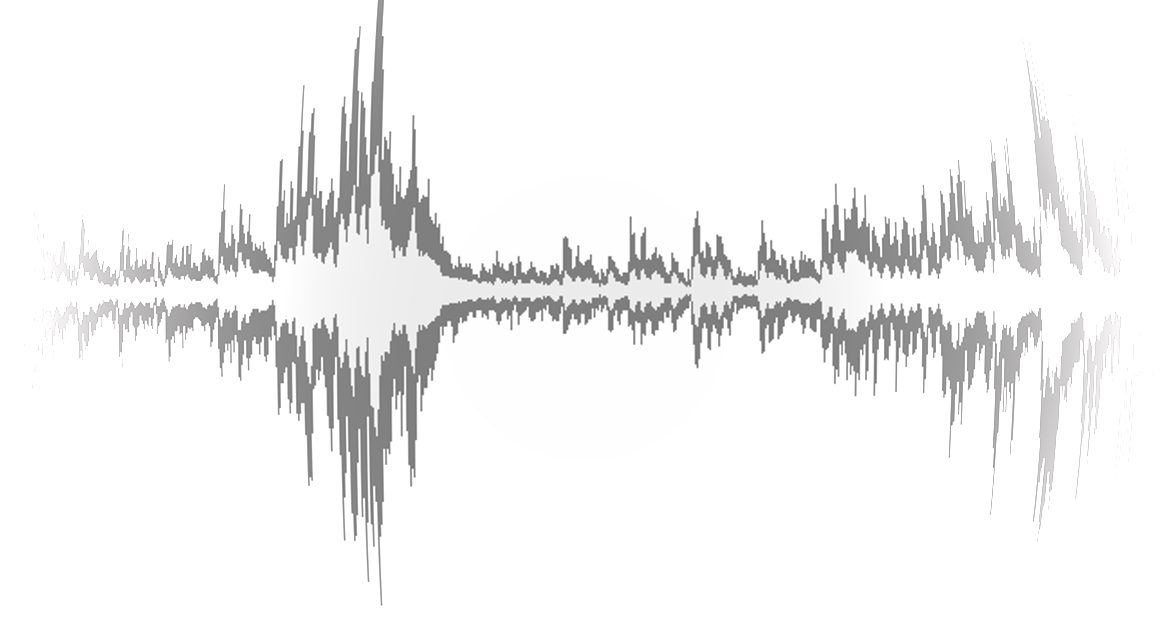
\includegraphics[width=\textwidth,height=3cm]{title}}


\begin{frame}
    \titlepage
    %\vspace{-5mm}
    \begin{flushright}
        \href{http://www.gtcmt.gatech.edu}{
\includegraphics[height=.8cm,keepaspectratio]{../shared/Logo_GTCMT_black}}
    \end{flushright}
\end{frame}


\section[intro]{introduction}
	\begin{frame}{filters}{introduction 1/2}
        \begin{block}{filter --- broad description}
            system that amplifies or attenuates certain components/aspects of a signal
        \end{block}
        \pause
        \bigskip
        \begin{block}{filter --- narrow description}
            linear time-invariant system for changing the magnitude and phase of specific frequency regions            
        \end{block}
        \pause
        \bigskip
        \begin{itemize}
            \item   example for other type of filters:
                \begin{itemize}
                    \item	adaptive  and time-variant (e.g., denoising)
                \end{itemize}
            \item	examples for ``real-world'' filters
                \begin{itemize}
                    \item	reverberation
                    \item	absorption
                    \item	echo
                \end{itemize}
        \end{itemize}
	\end{frame}
	\begin{frame}{filters}{introduction 2/2}
        \vspace{-5mm}
        \begin{columns}
            \column{.5\linewidth}
                \begin{itemize}
                    \item   \textbf{audio equalization}
                        \begin{itemize}
                            \item   parametric and graphic EQs
                        \end{itemize}
                    \smallskip
                    \item<2->   \textbf{removal} of unwanted components
                        \begin{itemize}
                            \item   remove DC, rumble, hum, hiss
                        \end{itemize}
                    \smallskip
                    \item<3->   \textbf{pre-emphasis/de-emphasis}
                        \begin{itemize}
                            \item   Vinyl
                            \item   old  noise reduction systems
                        \end{itemize}
                    \smallskip
                    \item<4->   \textbf{weighting} function
                        \begin{itemize}
                            \item   dBA, dBC, \ldots
                        \end{itemize}
                    \smallskip
                    \item<5->   (parameter) \textbf{smoothing}
                        \begin{itemize}
                            \item   smooth sudden changes
                        \end{itemize}
                \end{itemize}
                \vspace{70mm}
            \column{.5\linewidth}
                \only<1>{
                    \begin{figure}
                        \includegraphics[scale=.15]{graph/graphic_equalizer}
                    \end{figure}
                    \addreference{\href{https://en.wikipedia.org/wiki/File:Graphic_equalizer.jpg}{en.wikipedia.org/wiki/File:Graphic\_equalizer.jpg}}
                    }
                \only<2>{
                    \begin{figure}
                        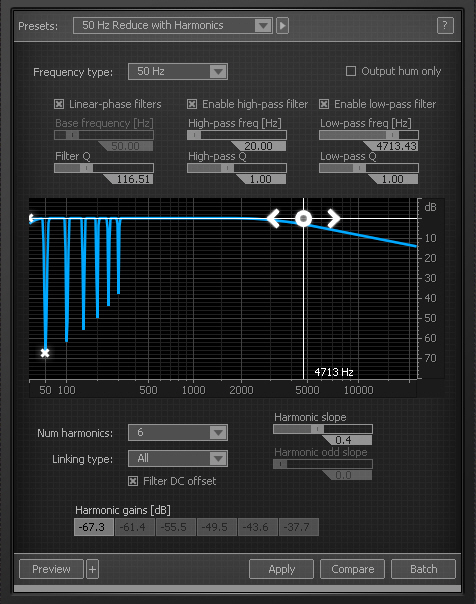
\includegraphics[scale=.25]{graph/hum_removal}
                    \end{figure}}
                \only<3>{
                    \begin{figure}
                        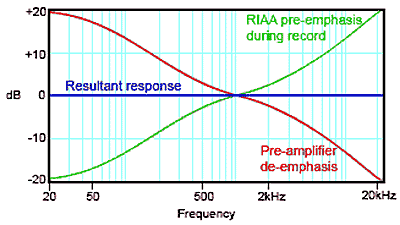
\includegraphics[scale=.4]{graph/riaa_emphasis}
                    \end{figure}
                    \addreference{\href{https://www.learnabout-electronics.org/Amplifiers/images/RIAA-curve.gif}{learnabout-electronics.org/Amplifiers/images/RIAA-curve.gif}}
                    }
                \only<4>{
                    \figwithmatlab{LoudnessWeighting}}
                \only<5>{
                    \figwithmatlab{Smoothing}}
        \end{columns}
	\end{frame}
 
    \begin{frame}{filters}{reminder: system theory}
        \begin{itemize}
            \item output of a system (filter) $y$ computed by \textbf{convolution} of input $x$ and impulse response $h$
                \begin{equation*}
                    y(t) = x(t) \ast h(t)   
                \end{equation*}
            \bigskip
            \item<2-> this is equivalent to a frequency domain multiplication 
                \begin{eqnarray*}
                    Y(\jom) &=& X(\jom) \cdot H(\jom)\\
                    H(\jom) &=& \frac{Y(\jom)}{X(\jom)}
                \end{eqnarray*}
            \bigskip
            \item<3-> \textbf{transfer function} $H(\jom)$ is complex, often represented as 
                \begin{itemize}
                    \item \textbf{magnitude} $|H(\jom)|$ and 
                    \item phase $\Phi_\mathrm{H}(\jom)$
                \end{itemize}
        \end{itemize}
    \end{frame}
   
    \section{equalization}
	\begin{frame}{filters}{common transfer function shapes}
            \question{what are typical filters/spectral filter shapes}

            \begin{columns}
            \column{.4\linewidth}
            \begin{itemize}
                \item   very common:
                    \begin{itemize}
                        \item   low/high pass
                    \end{itemize}
                \smallskip
                \item<3->   common for non-audio/non-parametric:
                    \begin{itemize}
                        \item   band pass/band stop
                    \end{itemize}
                \smallskip
                \item<4->   also common in audio apps:
                    \begin{itemize}
                        \item<4->   low/high shelving
                        \item<5->   peak filter
                        \item<6->   resonance/notch
                    \end{itemize}
            \end{itemize}
            \column{.65\linewidth}
                \vspace{-3mm}
                \only<2-3>{
                    \begin{figure}%
                        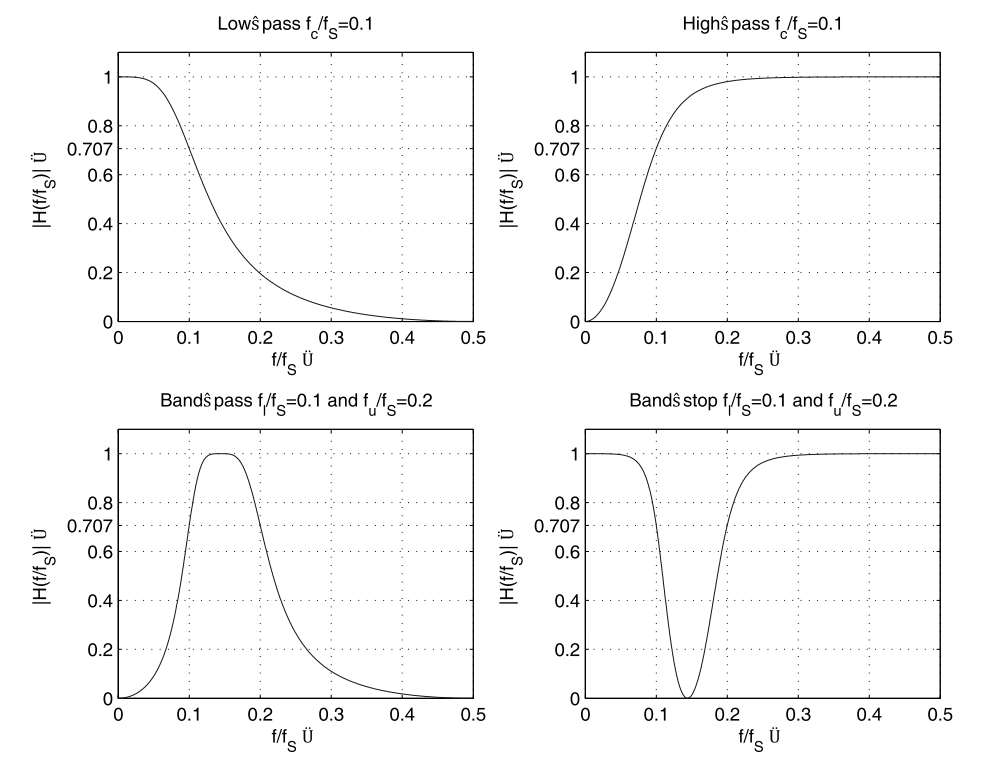
\includegraphics[width=.6\columnwidth]{graph/generalfilters_overview}%
                    \end{figure}
                }
                \only<4>{
                    \begin{figure}%
                        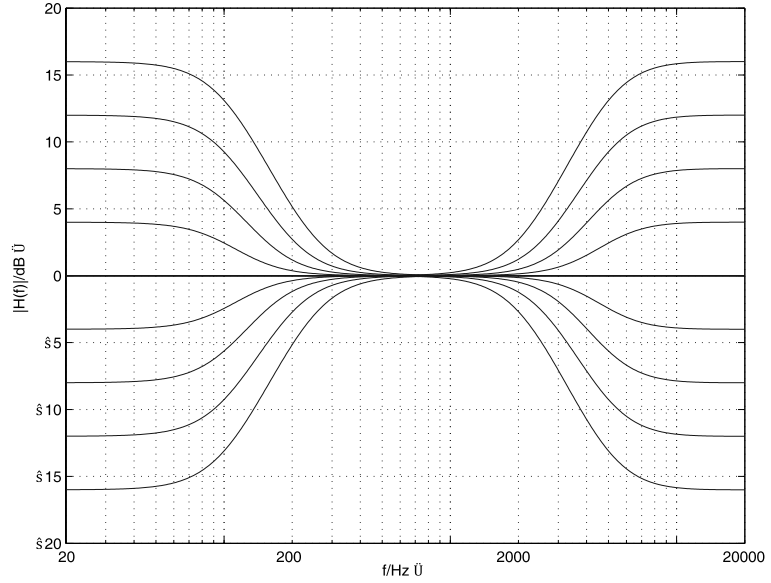
\includegraphics[width=.4\columnwidth]{graph/filter_shelving}%
                    \end{figure}
                }
                \only<5>{
                    \begin{figure}%
                        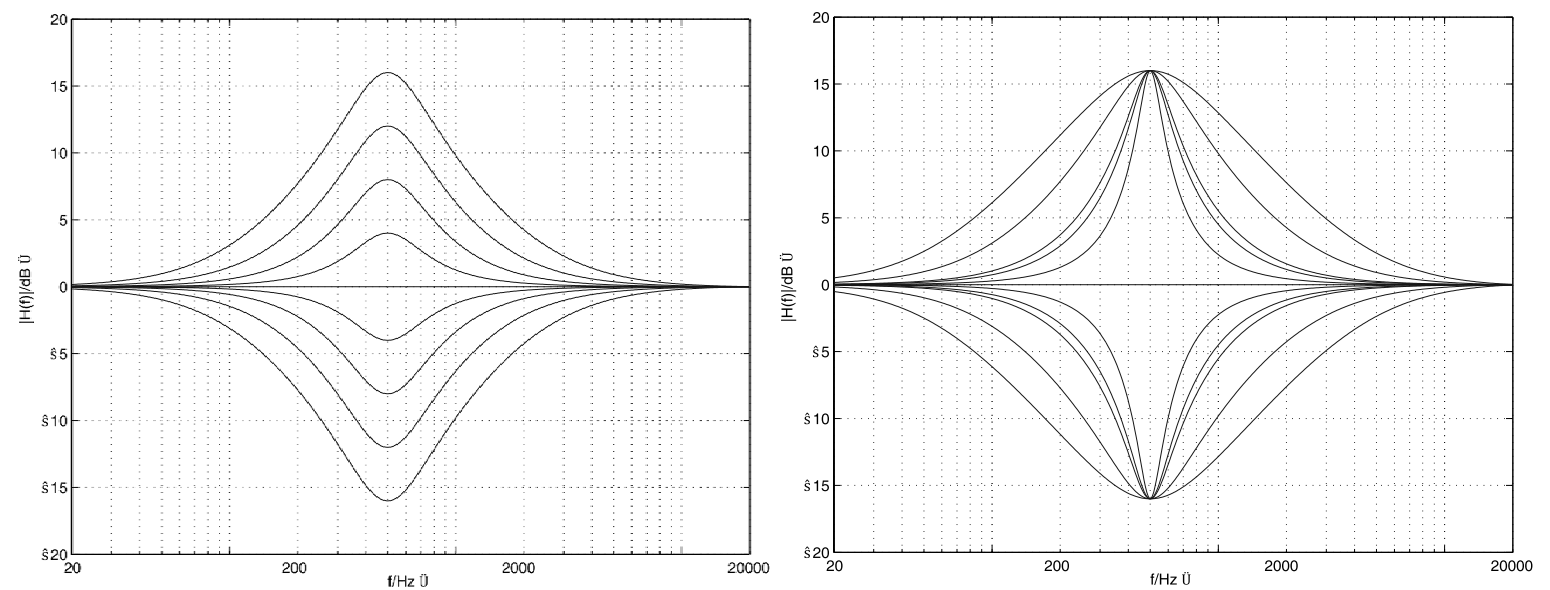
\includegraphics[width=\columnwidth]{graph/filter_peak}%
                    \end{figure}
                }
                \only<6>{
                    \begin{figure}%
                        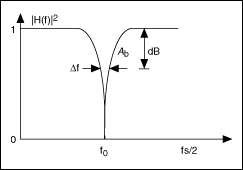
\includegraphics[width=.5\columnwidth]{graph/filter_notch}%
                    \end{figure}
                }
            \end{columns}
            \only<2-5>{\phantom{\footfullcite{zolzer_digital_2008}}}
    \end{frame}
	\begin{frame}{filters}{filters in series}
			\begin{figure}
				\centerline{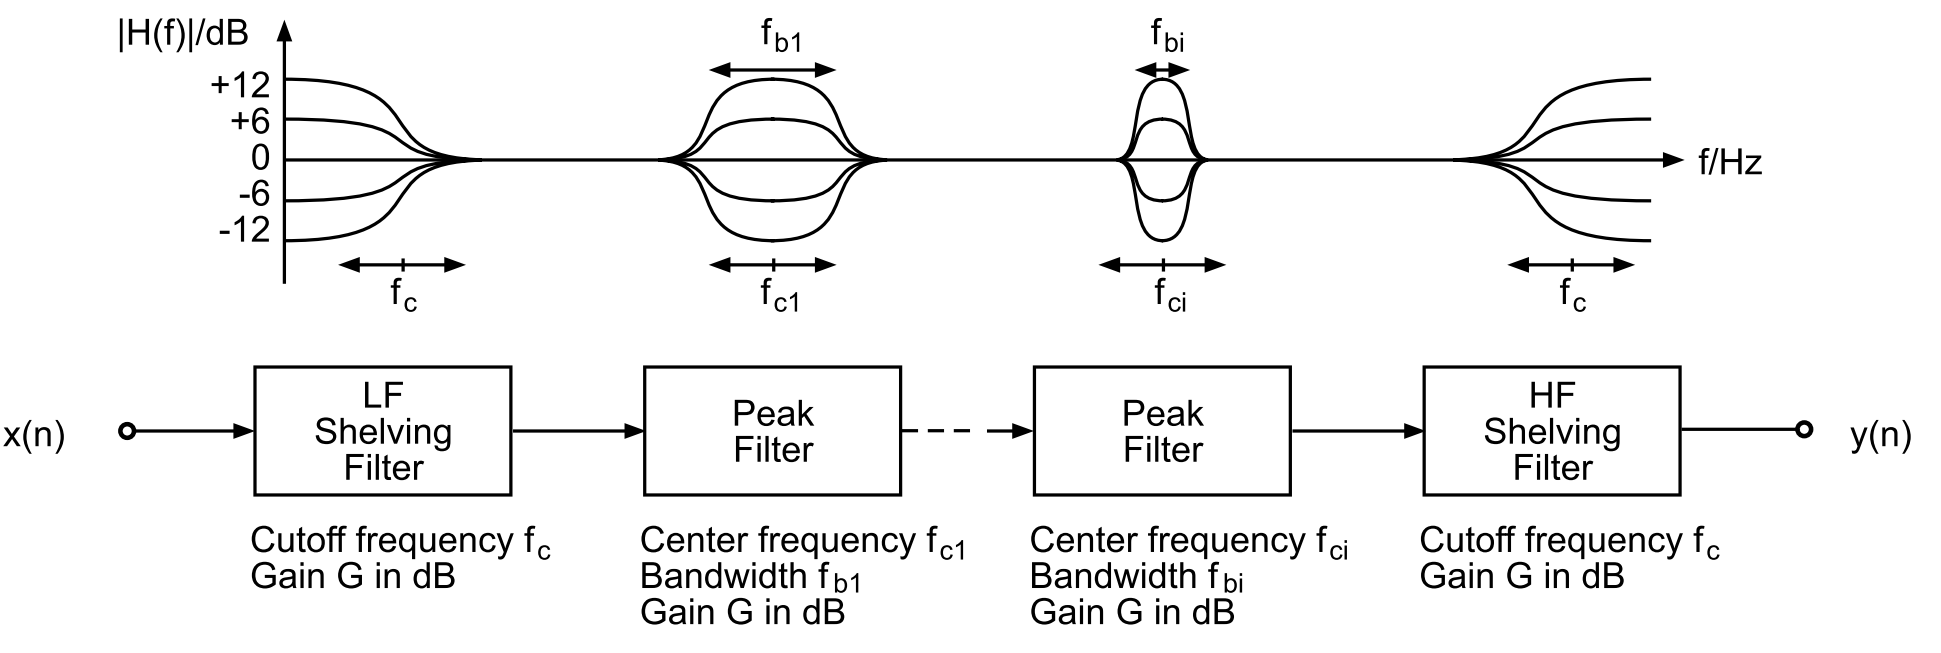
\includegraphics[width=\linewidth]{graph/zolzer_filterchain}}
			\end{figure}
            \phantom{\footfullcite{zolzer_digital_2008}}
	\end{frame}
    \begin{frame}{filters}{filter banks --- parallel connections}
        \vspace{-3mm}
        \only<1>{
        \begin{figure}%
            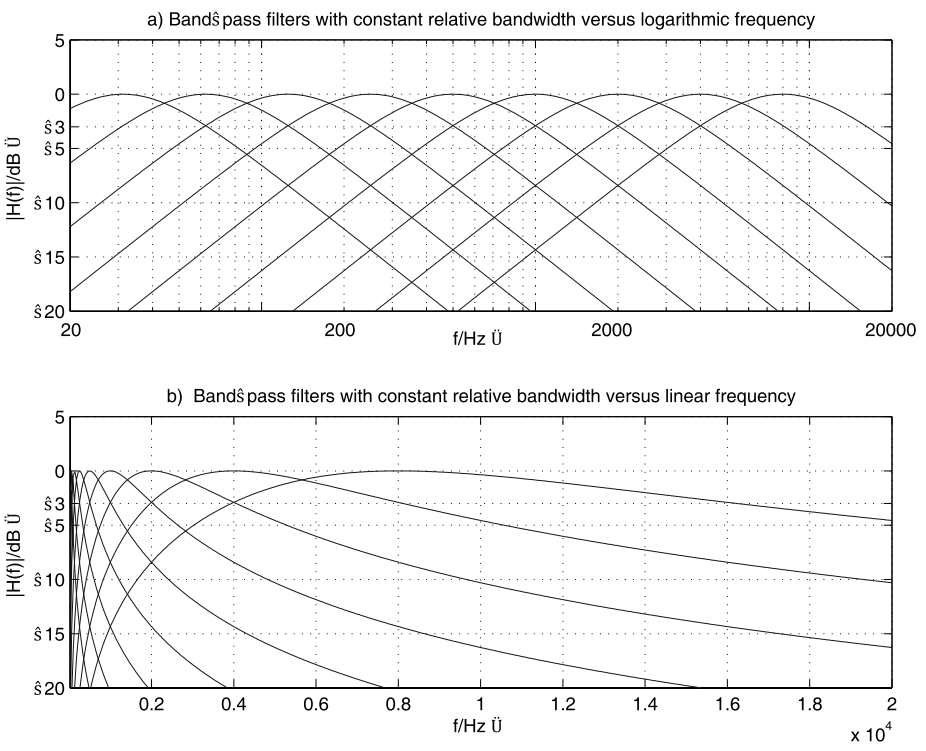
\includegraphics[width=.5\columnwidth]{graph/filterbank}%
        \end{figure}
        }
        \vspace{-2mm}
        \only<2>{
        \begin{figure}%
            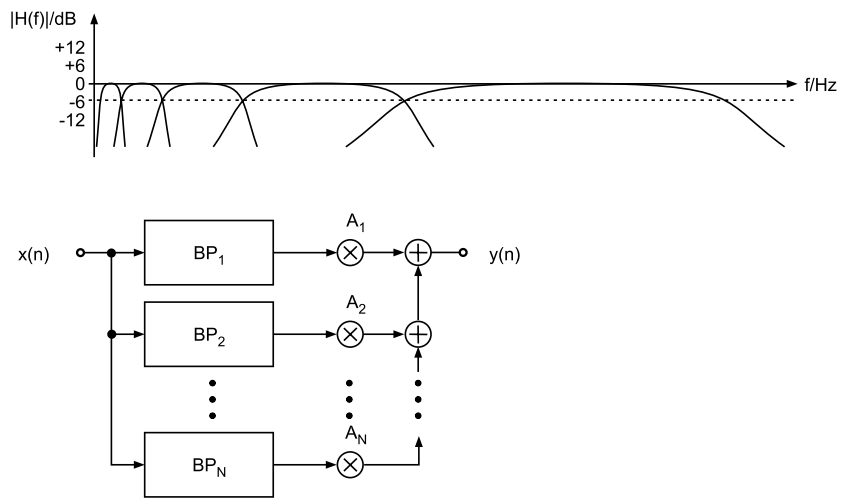
\includegraphics[width=.75\columnwidth]{graph/filterbank2}%
        \end{figure}
        }
            \phantom{\footfullcite{zolzer_digital_2008}}
    \end{frame}
    
\section{parameters}
        \begin{frame}{filters}{filter parameters --- lowpass/highpass}
            \vspace{-5mm}
            \begin{columns}
            \column{.5\linewidth}
                \begin{itemize}
                    \item   \textbf{cut-off} frequency $f_\mathrm{c}$
                        \begin{itemize}
                            \item   frequency marking the transition of pass to stop band
                            \item   \unit[-3]{dB} of pass band level
                        \end{itemize}
                    \smallskip
                    \item   \textbf{slope}/steepness
                        \begin{itemize}
                            \item   measured in dB/Octave or dB/Decade
                            \item   typically directly related to filter order
                        \end{itemize}
                    \smallskip
                    \item   sometimes: \textbf{resonance}    
                        \begin{itemize}
                            \item   level increase in narrow band around cut-off frequency
                        \end{itemize}
                \end{itemize}
            \column{.5\columnwidth}
                \begin{figure}%
                    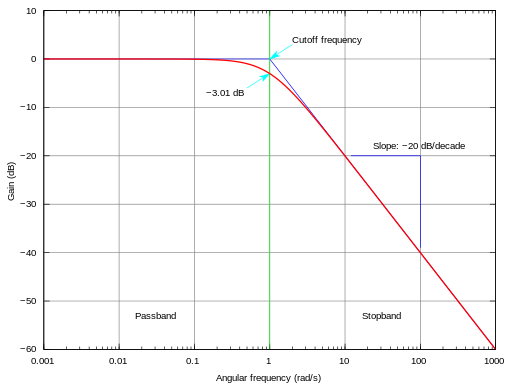
\includegraphics[width=.9\columnwidth]{graph/filter_parameters_lowpass}%
                \end{figure}
                \addreference{\href{https://en.wikipedia.org/wiki/File:Butterworth_response.svg}{en.wikipedia.org/wiki/File:Butterworth\_response.svg}}
            \end{columns}
        \end{frame}
        \begin{frame}{filters}{filter parameters --- bandpass/bandstop}
            \begin{columns}
            \column{.5\linewidth}
                \begin{itemize}
                    \item   \textbf{center} frequency $f_\mathrm{c}$
                        \begin{itemize}
                            \item   frequency marking the center of the pass or stop band
                        \end{itemize}
                    \smallskip
                    \item   \textbf{bandwidth} $\Delta B$
                        \begin{itemize}
                            \item   width of the pass band
                            \item   at \unit[-3]{dB} of max pass band level
                        \end{itemize}
                    \smallskip
                    \item   possibly: \textbf{slope}    
                        \begin{itemize}
                            \item   typically directly related to filter order
                        \end{itemize}
                \end{itemize}
            \column{.5\columnwidth}
                \begin{figure}%
                    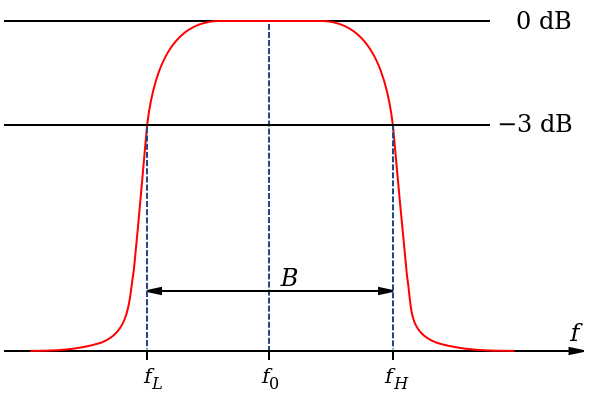
\includegraphics[width=.9\columnwidth]{graph/filter_parameters_bandpass}%
                \end{figure}
                \addreference{\href{https://en.wikipedia.org/wiki/File:Bandwidth_2.svg}{en.wikipedia.org/wiki/File:Bandwidth\_2.svg}}
            \end{columns}
        \end{frame}
        \begin{frame}{filters}{filter parameters --- peak}
            \begin{columns}
            \column{.5\linewidth}
                \begin{itemize}
                    \item   \textbf{center} frequency $f_\mathrm{c}$
                        \begin{itemize}
                            \item   frequency marking the center of the peak
                        \end{itemize}
                    \smallskip
                    \item   \textbf{Q factor} or \textbf{bandwidth} $\Delta B$
                        \begin{itemize}
                            \item   width of the bell
                            \item   at \unit[-3]{dB} of max gain
                            \[Q = \frac{f_\mathrm{c}}{\Delta B}\]
                        \end{itemize}
                    \smallskip
                    \item   \textbf{gain}    
                        \begin{itemize}
                            \item   amplification/attenuation in dB
                        \end{itemize}
                \end{itemize}
            \column{.5\columnwidth}
                \begin{figure}%
                    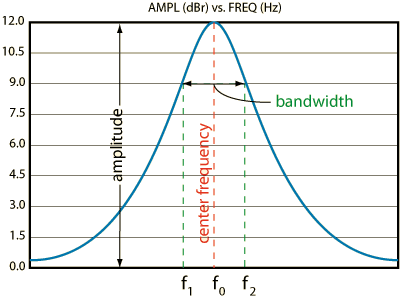
\includegraphics[width=.9\columnwidth]{graph/filter_parameters_peak}%
                \end{figure}
                \addreference{\href{http://www.sengpielaudio.com/FilterBandwidth09B.gif}{sengpielaudio.com/FilterBandwidth09B.gif}}
            \end{columns}
        \end{frame}
        \begin{frame}{filters}{filter parameters --- overview}
            \begin{footnotesize}
            \begin{table}%
            \begin{tabular}{l|ccccc}
                \textit{parameter} & \textbf{lowpass} & \textbf{low shelving} & \textbf{band pass} & \textbf{peak} & \textbf{resonance}\\ \hline
                \textit{frequency} &cut-off&cut-off&center&center&center\\
                \textit{bandwidth/Q} &res.\ gain&---&$\Delta B$& $Q$ &---\\
                %slope &dB/Oct&---&dB/Oct&---&---\\
                \textit{gain} &---&yes&---&yes&---
            \end{tabular}
            \end{table}
            \end{footnotesize}
        \end{frame}
        
\section{examples}	
	\begin{frame}{filters}{digital filter description}
		\begin{equation*}
			H(\mathrm{j}\omega) = \mathfrak{F}\{h(t)\}
		\end{equation*}


		filter is defined by its
		\begin{itemize}
			\item	complex transfer function $H(\mathrm{j}\omega)$, or its
			\item	impulse response $h(t)$, or its
			\item<2->	\textit{list of pole and zero positions in the Z-plane}
		\end{itemize}
	\end{frame}

	
	\begin{frame}{filters}{example 1}
        \setbeamercovered{invisible}

	        \begin{figure}
				\begin{center}
                	            \begin{picture}(50,30)
	
	                %boxes
	                \put(25,5){\framebox(7,6){\footnotesize{$z^{-1}$}}}
	
	                %lines horizontal
	                \put(5,20){\vector(1,0){22.5}}
	                \put(29.5,20){\vector(1,0){11.5}}
	                \put(43,20){\vector(1,0){10}}
	                
	                \put(15,8){\vector(1,0){10}}
	                \put(32,8){\line(1,0){10}}
	
	                %lines vertical
	                \put(15,20){\line(0,-1){12}}
	                \put(42,8){\vector(0,1){4}}
	                \put(42,14){\vector(0,1){5}}
	                
	                %circles
	                \put(27,19){$\otimes$}
	                \put(40.5,19){$\oplus$} % 42-20
	                \put(40.5,12){$\otimes$}
	                
	                \put(15,20){\circle*{1}}
	
	                %text
	                \put(26,24){\footnotesize{\shortstack[c]{$\nicefrac{1}{2}$}}}
	                \put(46,10){\footnotesize{\shortstack[c]{$\nicefrac{1}{2}$}}}
	
	                \put(4,22){\footnotesize{\shortstack[c]{x(i)}}}
	                \put(52,22){\footnotesize{\shortstack[c]{y(i)}}}
	
	            \end{picture}

				\end{center}
	        \end{figure}
        
        	\pause
            \begin{equation*}
        		y(i) = 0.5\cdot x(i) + 0.5\cdot x(i-1)
        	\end{equation*}
	\end{frame}	
	
	\begin{frame}{filters}{example 1: transfer function 1/2}
    	\begin{eqnarray*}
	        		y(i) &=& 0.5\cdot x(i) + 0.5\cdot x(i-1)\\
	        		H(z) &=& 0.5  + 0.5\cdot z^{-1}\\
	       	\pause
	        		H(j\omega) &=& 0.5  + 0.5\cdot e^{-j\omega}\\
	       	\pause
	       			|H(j\omega)| &=&0.5 \cdot \left| e^{-j\frac{\omega}{2}} \cdot \left( e^{j\frac{\omega}{2}} + e^{-j\frac{\omega}{2}}\right)\right| \\
	       	\pause
	       				&=&0.5 \cdot \underbrace{\left| e^{-j\frac{\omega}{2}}\right|}_{1} \cdot  \underbrace{\left|\left( e^{j\frac{\omega}{2}} + e^{-j\frac{\omega}{2}}\right)\right|}_{\left| 2\cos\left(\frac{\omega}{2}\right) \right|} \\
	       	\pause
	       	&=& \left| \cos\left(\frac{\omega}{2}\right) \right|
    	\end{eqnarray*}
	\end{frame}	
	
	\begin{frame}{filters}{example 1: transfer function 2/2}
		\begin{figure}
			\centerline{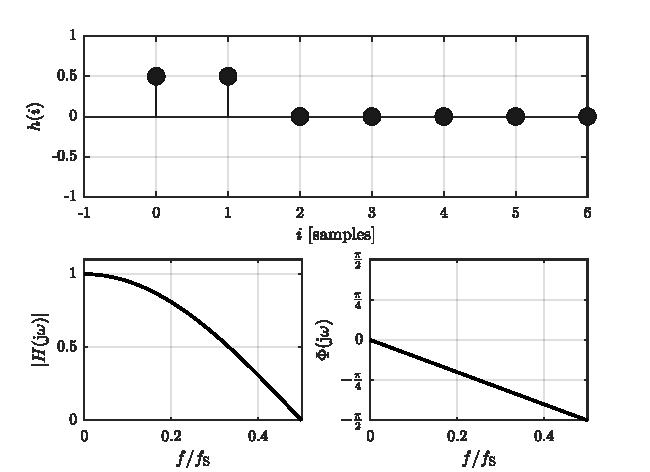
\includegraphics[scale=.8]{SimpleFilter-LP_FIR}}
		\end{figure}
        \addreference{matlab source: \href{https://github.com/alexanderlerch/MUSI-6202/blob/main/matlab/plotSimpleFilter.m}{plotSimpleFilter.m}}
	\end{frame}	
	
	\begin{frame}{filters}{example 2}
        \setbeamercovered{invisible}
        \begin{figure}
			\begin{center}
                            \begin{picture}(50,30)

                %boxes
                \put(25,5){\framebox(7,6){\footnotesize{$z^{-1}$}}}

                %lines horizontal
                \put(5,20){\vector(1,0){22.5}}
                \put(29.5,20){\vector(1,0){11.5}}
                \put(43,20){\vector(1,0){10}}
                
                \put(15,8){\vector(1,0){10}}
                \put(32,8){\line(1,0){10}}

                %lines vertical
                \put(15,20){\line(0,-1){12}}
                \put(42,8){\vector(0,1){4}}
                \put(42,14){\vector(0,1){5}}
                
                %circles
                \put(27,19){$\otimes$}
                \put(40.5,19){$\oplus$} % 42-20
                \put(40.5,12){$\otimes$}
                
                \put(15,20){\circle*{1}}

                %text
                \put(26,24){\footnotesize{\shortstack[c]{$\nicefrac{1}{2}$}}}
                \put(46,10){\footnotesize{\shortstack[c]{$-\nicefrac{1}{2}$}}}

                \put(4,22){\footnotesize{\shortstack[c]{x(i)}}}
                \put(52,22){\footnotesize{\shortstack[c]{y(i)}}}

            \end{picture}

			\end{center}
        \end{figure}
        \pause
    	\begin{eqnarray*}
    		y(i) &=& 0.5\cdot x(i) - 0.5\cdot x(i-1)\\
    		H(z) &=& 0.5  - 0.5\cdot z^{-1}\\
    	\pause
    		|H(j\omega)| &=& \left| \sin\left(\frac{\omega}{2}\right) \right|
    	\end{eqnarray*}
	\end{frame}	
	
	\begin{frame}{filters}{example 2: transfer function}
		\begin{figure}
			\centerline{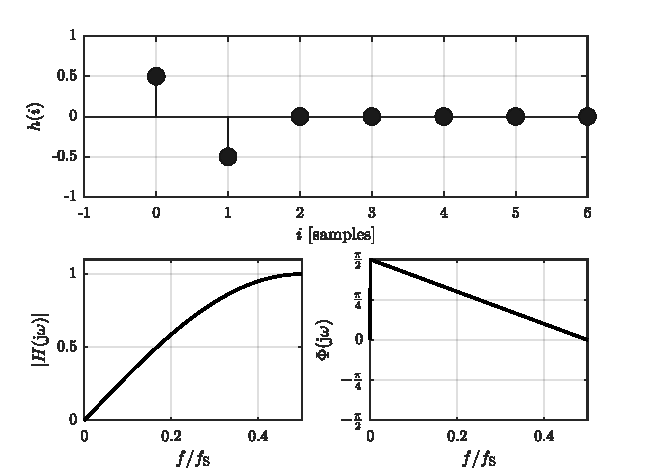
\includegraphics[scale=.8]{SimpleFilter-HP_FIR}}
		\end{figure}
        \addreference{matlab source: \href{https://github.com/alexanderlerch/MUSI-6202/blob/main/matlab/plotSimpleFilter.m}{plotSimpleFilter.m}}
	\end{frame}	
	
	\begin{frame}{filters}{example 3}
        \setbeamercovered{invisible}
       \begin{figure}[!hbt]
			\begin{center}
                            \begin{picture}(50,30)

                %boxes
                \put(25,5){\framebox(7,6){\footnotesize{$z^{-N}$}}}

                %lines horizontal
                \put(5,20){\vector(1,0){22.5}}
                \put(29.5,20){\vector(1,0){11.5}}
                \put(43,20){\vector(1,0){10}}
                
                \put(15,8){\vector(1,0){10}}
                \put(32,8){\line(1,0){10}}

                %lines vertical
                \put(15,20){\line(0,-1){12}}
                \put(42,8){\vector(0,1){4}}
                \put(42,14){\vector(0,1){5}}
                
                %circles
                \put(27,19){$\otimes$}
                \put(40.5,19){$\oplus$} % 42-20
                \put(40.5,12){$\otimes$}
                
                \put(15,20){\circle*{1}}

                %text
                \put(26,24){\footnotesize{\shortstack[c]{$\nicefrac{1}{2}$}}}
                \put(46,10){\footnotesize{\shortstack[c]{$-\nicefrac{1}{2}$}}}

                \put(4,22){\footnotesize{\shortstack[c]{x(i)}}}
                \put(52,22){\footnotesize{\shortstack[c]{y(i)}}}

            \end{picture}

			\end{center}
        \end{figure}
		\pause      
    	\begin{eqnarray*}
    		y(i) &=& 0.5\cdot x(i) - 0.5\cdot x(i-N)\\
    		H(z) &=& 0.5  - 0.5\cdot z^{-N}\\
			\pause
    		|H(j\omega)| &=& 0.5\cdot\left| e^{-j\frac{N\omega}{2}} \cdot \left(e^{j\frac{N\omega}{2}} - e^{-j\frac{N\omega}{2}} \right) \right|\\
			\pause
    		 &=& \left| \sin\left(\frac{N\omega}{2}\right) \right|
    	\end{eqnarray*}
	\end{frame}	
	
	\begin{frame}{filters}{example 3: transfer function}
		\begin{figure}
			\centerline{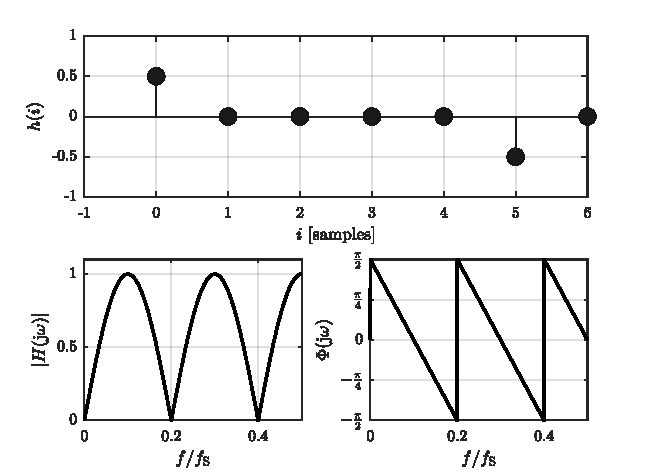
\includegraphics[scale=.8]{SimpleFilter-CB_FIR}}
		\end{figure}
        \addreference{matlab source: \href{https://github.com/alexanderlerch/MUSI-6202/blob/main/matlab/plotSimpleFilter.m}{plotSimpleFilter.m}}
	\end{frame}	
	
	\begin{frame}{filters}{example 4}
        \setbeamercovered{invisible}
        \begin{columns}
        \column{.6\linewidth}
        \begin{figure}
			\begin{center}
                            \begin{picture}(50,70)

                %boxes
                \put(25,50){\framebox(7,6){\footnotesize{$z^{-1}$}}}
                \put(25,38){\framebox(7,6){\footnotesize{$z^{-2}$}}}
                \put(28,28){\shortstack[c]{$\vdots$}}
                \put(21,14){\framebox(14,6){\footnotesize{$z^{-(\mathcal{J}-1)}$}}}

                %lines horizontal
                \put(5,65){\vector(1,0){22.5}}
                \put(29.5,65){\vector(1,0){11.5}}
                \put(43,65){\vector(1,0){10}}
                
                \put(15,53){\vector(1,0){10}}
                \put(32,53){\vector(1,0){4}}
                \put(38,53){\vector(1,0){3}}
                
                \put(15,41){\vector(1,0){10}}
                \put(32,41){\vector(1,0){4}}
                \put(38,41){\vector(1,0){3}}
                
                \put(15,29){\vector(1,0){10}}
                \put(32,29){\vector(1,0){4}}
                \put(38,29){\vector(1,0){3}}
                
                \put(15,17){\vector(1,0){6}}
                \put(35,17){\line(1,0){7}}

                %lines vertical
                \put(15,65){\line(0,-1){48}}
                \put(42,54){\vector(0,1){10}}
                %\put(42,60){\vector(0,1){4}}
                
                \put(42,42){\vector(0,1){10}}
                %\put(42,48){\vector(0,1){4}}
                
                \put(42,30){\vector(0,1){10}}
                %\put(42,36){\vector(0,1){4}}
                
                \put(42,17){\vector(0,1){5}}
                \put(42,24){\vector(0,1){4}}
                
                %circles
                \put(27,64){$\otimes$}
                \put(40.5,64){$\oplus$} % 42-20
                \put(40.5,52){$\oplus$} % 42-20
                \put(40.5,40){$\oplus$} % 42-20
                \put(40.5,28){$\oplus$} % 42-20
                
                \put(35.5,52){$\otimes$}
                \put(35.5,40){$\otimes$}
                \put(35.5,28){$\otimes$}
                \put(40.5,22){$\otimes$}
                
                \put(15,65){\circle*{1}}
                \put(15,53){\circle*{1}}
                \put(15,41){\circle*{1}}
                \put(15,29){\circle*{1}}

                %text
                \put(26,69){\footnotesize{\shortstack[c]{$\nicefrac{1}{\mathcal{J}}$}}}
                \put(35,57){\footnotesize{\shortstack[c]{$\nicefrac{1}{\mathcal{J}}$}}}
                \put(35,45){\footnotesize{\shortstack[c]{$\nicefrac{1}{\mathcal{J}}$}}}
                \put(35,33){\footnotesize{\shortstack[c]{$\nicefrac{1}{\mathcal{J}}$}}}
                \put(44,21){\footnotesize{\shortstack[c]{$\nicefrac{1}{\mathcal{J}}$}}}

                \put(4,67){\footnotesize{\shortstack[c]{x(i)}}}
                \put(52,67){\footnotesize{\shortstack[c]{y(i)}}}

            \end{picture}

			\end{center}
        \end{figure}
        
        \column{.4\linewidth}
        \only<2>{
    	\begin{equation*}
    		y(i) = \frac{1}{\mathcal{J}}\sum_{j=0}^{\mathcal{J}-1} x(i-j)
    	\end{equation*}
        }
        \end{columns}
	\end{frame}
	\begin{frame}{filters}{example 4: transfer function}
        \vspace{-10mm}
        \begin{columns}
        \column{.7\linewidth}
		\begin{figure}
			\centerline{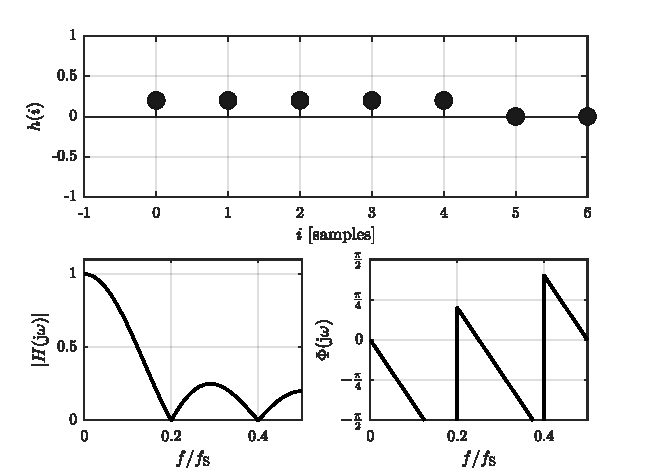
\includegraphics[scale=.8]{SimpleFilter-MA_FIR}}
		\end{figure}
        \addreference{matlab source: \href{https://github.com/alexanderlerch/MUSI-6202/blob/main/matlab/plotSimpleFilter.m}{plotSimpleFilter.m}}
        \column{.3\linewidth}
    	\begin{equation*}
    		H(j\omega) = e^{-\mathrm{j}\mathcal{J}\frac{\omega}{2}}\frac{\sin\left(\mathcal{J}\cdot\frac{\omega}{2} \right)}{\mathcal{J}\cdot\sin\left(\frac{\omega}{2} \right)}
    	\end{equation*}
        \end{columns}

	\end{frame}	
	\begin{frame}{filters}{example 4: recursive implementation}
		\begin{eqnarray*}
			y(i) &=& \sum\limits_{j=0}^{\mathcal{J}-1}{\frac{1}{\mathcal{J}}\cdot x(i-j)}\nonumber\\
			\pause
			&=& \frac{1}{\mathcal{J}}\cdot \big(x(i) - x(i-\mathcal{J})\big) + \underbrace{\sum\limits_{j=1}^{\mathcal{J}}{\frac{1}{\mathcal{J}}\cdot x(i-j)}}_{y(i-1)}\nonumber\\
			\pause
			&=& \frac{1}{\mathcal{J}}\cdot \big(x(i) - x(i-\mathcal{J})\big) + y(i-1) 
		\end{eqnarray*} 
		\pause
		\textcolor{gtgold}{not applicable with windowed coefficients!}
	\end{frame}
	\begin{frame}{filters}{example 5}
        \setbeamercovered{invisible}
	        \begin{figure}[!hbt]
				\begin{center}
                	            \begin{picture}(50,30)
	
	                %boxes
	                \put(25,5){\framebox(7,6){\footnotesize{$z^{-1}$}}}
	
	                %lines horizontal
	                \put(0,20){\vector(1,0){6}}
	                \put(8,20){\vector(1,0){47}}
	                
	                \put(15,8){\line(1,0){10}}
	                \put(42,8){\vector(-1,0){10}}
	
	                %lines vertical
	                \put(42,20){\line(0,-1){12}}
	                \put(15,8){\vector(0,1){4}}
	                \put(15,14){\vector(0,1){5}}
	                
	                %circles
	                \put(5.5,19){$\otimes$}
	                \put(13.5,19){$\oplus$} % 15-20
	                \put(13.5,12){$\otimes$}
	                
	                \put(42,20){\circle*{1}}
	
	                %text
	                \put(4,22){\footnotesize{\shortstack[c]{$(1-\alpha)$}}}
	                \put(11,10){\footnotesize{\shortstack[c]{$\alpha$}}}
	
	                \put(-2,22){\footnotesize{\shortstack[c]{x(i)}}}
	                \put(52,22){\footnotesize{\shortstack[c]{y(i)}}}
	
	            \end{picture}

				\end{center}
	        \end{figure}
            \pause
        	\begin{eqnarray*}
        		y(i) &=& (1-\alpha)\cdot x(i) + \alpha\cdot y(i-1)\\
        			&=& x(i) + \alpha \cdot (y(i-1) - x(i))
        	\end{eqnarray*}
	\end{frame}
	
	\begin{frame}{Example 5: transfer function 1/2}
    	\begin{eqnarray*}
        		y(i) &=& (1-\alpha)\cdot x(i) + \alpha\cdot y(i-1)\\
        		H(z) &=& \frac{1-\alpha}{1-\alpha z^{-1}}\\
        \pause
        		H(j\omega) &=& \frac{1-\alpha}{1-\alpha e^{-j\omega}}\\
        \pause
        		|H(j\omega)| &=& \left|\frac{1-\alpha}{1-\alpha e^{-j\omega}}\right| \\
        \pause
        		&=&\frac{1-\alpha}{\sqrt{\left(1 + \alpha^2 - 2\alpha\cos(\omega)\right)}} 
    	\end{eqnarray*}
	\end{frame}
	\begin{frame}{filters}{example 5: transfer function 2/2}
		\begin{figure}
			\centerline{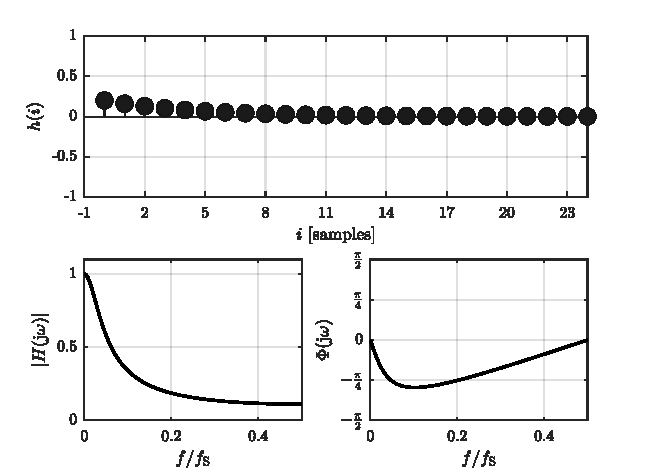
\includegraphics[scale=.8]{SimpleFilter-LP_IIR}}
		\end{figure}
        \addreference{matlab source: \href{https://github.com/alexanderlerch/MUSI-6202/blob/main/matlab/plotSimpleFilter.m}{plotSimpleFilter.m}}
	\end{frame}
	\begin{frame}{filters}{example 6}
        \begin{figure}[!hbt]
			\begin{center}
                            \begin{picture}(50,30)

                %boxes
                \put(25,5){\framebox(7,6){\footnotesize{$z^{-N}$}}}

                %lines horizontal
                \put(0,20){\vector(1,0){14}}
                \put(16,20){\vector(1,0){32}}
                \put(50,20){\vector(1,0){5}}
                
                \put(15,8){\line(1,0){10}}
                \put(42,8){\vector(-1,0){10}}

                %lines vertical
                \put(42,20){\line(0,-1){12}}
                \put(15,8){\vector(0,1){4}}
                \put(15,14){\vector(0,1){5}}
                
                %circles
                \put(47.5,19){$\otimes$}
                \put(13.5,19){$\oplus$} % 15-20
                \put(13.5,12){$\otimes$}
                
                \put(42,20){\circle*{1}}

                %text
                \put(43,22){\footnotesize{\shortstack[c]{$b_0$}}}
                \put(8,10){\footnotesize{\shortstack[c]{$-a_N$}}}

                \put(-2,22){\footnotesize{\shortstack[c]{x(i)}}}
                \put(52,22){\footnotesize{\shortstack[c]{y(i)}}}

            \end{picture}

			\end{center}
        \end{figure}
    	\begin{equation*}
    		y(i) = b_0\cdot x(i) - a_N\cdot y(i-N)
    	\end{equation*}
	\end{frame}
	\begin{frame}{filters}{example 6: transfer function}
        \vspace{-10mm}
        \begin{columns}
        \column{.7\linewidth}
		\begin{figure}
			\centerline{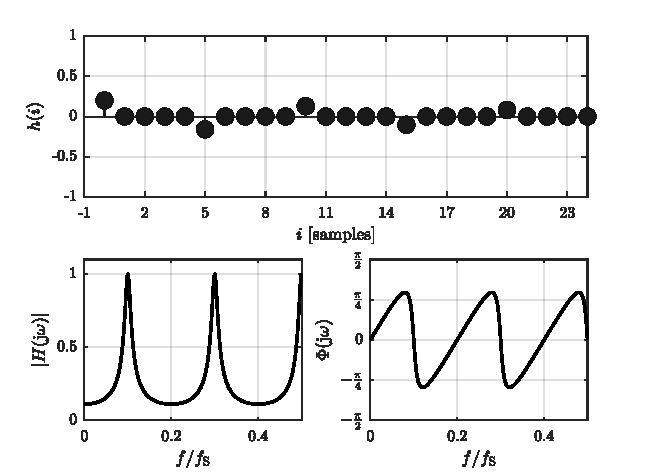
\includegraphics[scale=.8]{SimpleFilter-CB_IIR}}
		\end{figure}
        \addreference{matlab source: \href{https://github.com/alexanderlerch/MUSI-6202/blob/main/matlab/plotSimpleFilter.m}{plotSimpleFilter.m}}
        \column{.3\linewidth}
    	\begin{equation*}
    		H(j\omega) = \frac{b_0}{1-a_N\cdot e^{-j\omega N}}
    	\end{equation*}
        \end{columns}
	\end{frame}
	\begin{frame}{filters}{biquad: structure}
        \vspace{-3mm}
		\begin{figure}
			\centerline{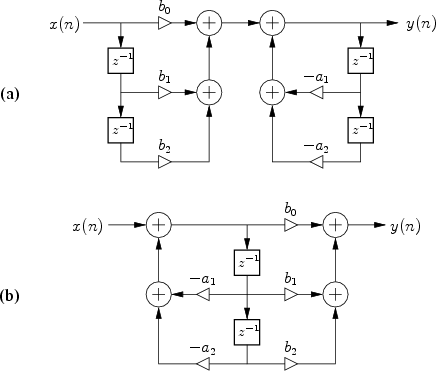
\includegraphics[scale=.3]{graph/general_biquad_jos}}
		    \label{fig:general_biquad}
		\end{figure}
		\pause
		\vspace{-3mm}
		\begin{eqnarray*}
			\text{diff eq}: y(i) 	&=& \sum_{k=0}^{K_1}{b_k\cdot x(i-k)} + \sum_{k=1}^{K_2}{-a_k\cdot y(i-k)} \nonumber\\
			\text{trans. fct}: H(z) 	&=& \frac{Y(z)}{X(z)} =  \frac{\sum_{k=0}^{K_1}{b_k\cdot z^{-k}}}{1 + \sum_{k=1}^{K_2}{a_k\cdot z^{-k}}} 
		\end{eqnarray*}
	\end{frame}

	\section{summary}	
        \begin{frame}{filters}{summary}
            \vspace{-3mm}
            \begin{itemize}
                \item   filter (equalization) can be used for various tasks
                    \begin{itemize}
                        \item   changing the sound quality of a signal
                        \item   hiding unwanted frequency components
                        \item   smoothing
                        \item   processing for measurement and transmission
                    \end{itemize}
                \item<2->   most common audio filter types are
                    \begin{itemize}
                        \item   low/high pass
                        \item   peak
                        \item   shelving
                    \end{itemize}
                \item<3->   filter parameters include
                    \begin{itemize}
                        \item   frequency (mid, cutoff)
                        \item   bandwidth or Q
                        \item   gain
                    \end{itemize}
                \item<4->   filter orders
                    \begin{itemize}
                        \item   typical orders are 1st, 2nd, maybe 4th
                        \item   higher order give more flexibility wrt transfer function
                        \item   higher orders are difficult to design and control
                        \item   higher orders can be split into multiple low order filters
                    \end{itemize}
            \end{itemize}
        \end{frame}
 

\end{document}

